\PassOptionsToPackage{dvipsnames,table}{xcolor}
\documentclass[10pt]{beamer}
\usepackage{Cours}

\begin{document}

%QCM de NSI \QNSI{Question}{R1}{R2}{R3}{R4}
\newcommand{\QNSI}[5]{
#1
\begin{enumerate}
\item #2
\item #3
\item #4
\item #5
\end{enumerate}
}


\newcounter{numchap}
\setcounter{numchap}{1}
\newcounter{numframe}
\setcounter{numframe}{0}
\newcommand{\mframe}[1]{\frametitle{#1} \addtocounter{numframe}{1}}
\newcommand{\cnum}{\fbox{\textcolor{yellow}{\textbf{C\thenumchap}}}~}

\definecolor{grispale}{gray}{0.95}


\definecolor{grispale}{gray}{0.95}
\newcommand{\htmlmode}{\lstset{language=html,numbers=left, tabsize=2, frame=single, breaklines=true, keywordstyle=\ttfamily, basicstyle=\small,
   numberstyle=\tiny\ttfamily, framexleftmargin=0mm, backgroundcolor=\color{grispale}, xleftmargin=12mm,showstringspaces=false}}
\newcommand{\pythonmode}{\lstset{language=python,linewidth=\linewidth,numbers=left, tabsize=2, frame=single, breaklines=true, keywordstyle=\ttfamily\color{blue}, basicstyle=\small,
   numberstyle=\tiny\ttfamily, framexleftmargin=-2mm,numbersep=-0.5mm,backgroundcolor=\color{grispale}, xleftmargin=-1mm, showstringspaces=false,commentstyle=\color{gray},stringstyle=\color{OliveGreen},morekeywords={setheading,goto,backward,forward,left,right,pendown,penup,pensize,color,speed,hideturtle,showturtle,forward}}}
\newcommand{\bashmode}{\lstset{language=bash,numbers=left, tabsize=2, frame=single, breaklines=true, basicstyle=\ttfamily,
   numberstyle=\tiny\ttfamily, framexleftmargin=0mm, backgroundcolor=\color{grispale}, xleftmargin=12mm, showstringspaces=false}}
\newcommand{\exomode}{\lstset{language=python,numbers=left, tabsize=2, frame=single, breaklines=true, basicstyle=\ttfamily,
   numberstyle=\tiny\ttfamily, framexleftmargin=13mm, xleftmargin=12mm, basicstyle=\small, showstringspaces=false}}
   
   
  \lstset{%
        inputencoding=utf8,
        extendedchars=true,
        literate=%
        {é}{{\'{e}}}1
        {è}{{\`{e}}}1
        {ê}{{\^{e}}}1
        {ë}{{\¨{e}}}1
        {É}{{\'{E}}}1
        {Ê}{{\^{E}}}1
        {û}{{\^{u}}}1
        {ù}{{\`{u}}}1
        {ú}{{\'{u}}}1
        {â}{{\^{a}}}1
        {à}{{\`{a}}}1
        {á}{{\'{a}}}1
        {ã}{{\~{a}}}1
        {Á}{{\'{A}}}1
        {Â}{{\^{A}}}1
        {Ã}{{\~{A}}}1
        {ç}{{\c{c}}}1
        {Ç}{{\c{C}}}1
        {õ}{{\~{o}}}1
        {ó}{{\'{o}}}1
        {ô}{{\^{o}}}1
        {Õ}{{\~{O}}}1
        {Ó}{{\'{O}}}1
        {Ô}{{\^{O}}}1
        {î}{{\^{i}}}1
        {Î}{{\^{I}}}1
        {í}{{\'{i}}}1
        {Í}{{\~{Í}}}1
}

%tei pour placer les images
%tei{nom de l’image}{échelle de l’image}{sens}{texte a positionner}
%sens ="1" (droite) ou "2" (gauche)
\newlength{\ltxt}
\newcommand{\tei}[4]{
\setlength{\ltxt}{\linewidth}
\setbox0=\hbox{\includegraphics[scale=#2]{#1}}
\addtolength{\ltxt}{-\wd0}
\addtolength{\ltxt}{-10pt}
\ifthenelse{\equal{#3}{1}}{
\begin{minipage}{\wd0}
\includegraphics[scale=#2]{#1}
\end{minipage}
\hfill
\begin{minipage}{\ltxt}
#4
\end{minipage}
}{
\begin{minipage}{\ltxt}
#4
\end{minipage}
\hfill
\begin{minipage}{\wd0}
\includegraphics[scale=#2]{#1}
\end{minipage}
}
}

%Juxtaposition d'une image pspciture et de texte 
%#1: = code pstricks de l'image
%#2: largeur de l'image
%#3: hauteur de l'image
%#4: Texte à écrire
\newcommand{\ptp}[4]{
\setlength{\ltxt}{\linewidth}
\addtolength{\ltxt}{-#2 cm}
\addtolength{\ltxt}{-0.1 cm}
\begin{minipage}[b][#3 cm][t]{\ltxt}
#4
\end{minipage}\hfill
\begin{minipage}[b][#3 cm][c]{#2 cm}
#1
\end{minipage}\par
}



%Macros pour les graphiques
\psset{linewidth=0.5\pslinewidth,PointSymbol=x}
\setlength{\fboxrule}{0.5pt}
\newcounter{tempangle}

%Marque la longueur du segment d'extrémité  #1 et  #2 avec la valeur #3, #4 est la distance par rapport au segment (en %age de la valeur de celui ci) et #5 l'orientation du marquage : +90 ou -90
\newcommand{\afflong}[5]{
\pstRotation[RotAngle=#4,PointSymbol=none,PointName=none]{#1}{#2}[X] 
\pstHomO[PointSymbol=none,PointName=none,HomCoef=#5]{#1}{X}[Y]
\pstTranslation[PointSymbol=none,PointName=none]{#1}{#2}{Y}[Z]
 \ncline{|<->|,linewidth=0.25\pslinewidth}{Y}{Z} \ncput*[nrot=:U]{\footnotesize{#3}}
}
\newcommand{\afflongb}[3]{
\ncline{|<->|,linewidth=0}{#1}{#2} \naput*[nrot=:U]{\footnotesize{#3}}
}

%Construis le point #4 situé à #2 cm du point #1 avant un angle #3 par rapport à l'horizontale. #5 = liste de paramètre
\newcommand{\lsegment}[5]{\pstGeonode[PointSymbol=none,PointName=none](0,0){O'}(#2,0){I'} \pstTranslation[PointSymbol=none,PointName=none]{O'}{I'}{#1}[J'] \pstRotation[RotAngle=#3,PointSymbol=x,#5]{#1}{J'}[#4]}
\newcommand{\tsegment}[5]{\pstGeonode[PointSymbol=none,PointName=none](0,0){O'}(#2,0){I'} \pstTranslation[PointSymbol=none,PointName=none]{O'}{I'}{#1}[J'] \pstRotation[RotAngle=#3,PointSymbol=x,#5]{#1}{J'}[#4] \pstLineAB{#4}{#1}}

%Construis le point #4 situé à #3 cm du point #1 et faisant un angle de  90° avec la droite (#1,#2) #5 = liste de paramètre
\newcommand{\psegment}[5]{
\pstGeonode[PointSymbol=none,PointName=none](0,0){O'}(#3,0){I'}
 \pstTranslation[PointSymbol=none,PointName=none]{O'}{I'}{#1}[J']
 \pstInterLC[PointSymbol=none,PointName=none]{#1}{#2}{#1}{J'}{M1}{M2} \pstRotation[RotAngle=-90,PointSymbol=x,#5]{#1}{M1}[#4]
  }
  
%Construis le point #4 situé à #3 cm du point #1 et faisant un angle de  #5° avec la droite (#1,#2) #6 = liste de paramètre
\newcommand{\mlogo}[6]{
\pstGeonode[PointSymbol=none,PointName=none](0,0){O'}(#3,0){I'}
 \pstTranslation[PointSymbol=none,PointName=none]{O'}{I'}{#1}[J']
 \pstInterLC[PointSymbol=none,PointName=none]{#1}{#2}{#1}{J'}{M1}{M2} \pstRotation[RotAngle=#5,PointSymbol=x,#6]{#1}{M2}[#4]
  }

% Construis un triangle avec #1=liste des 3 sommets séparés par des virgules, #2=liste des 3 longueurs séparés par des virgules, #3 et #4 : paramètre d'affichage des 2e et 3 points et #5 : inclinaison par rapport à l'horizontale
%autre macro identique mais sans tracer les segments joignant les sommets
\noexpandarg
\newcommand{\Triangleccc}[5]{
\StrBefore{#1}{,}[\pointA]
\StrBetween[1,2]{#1}{,}{,}[\pointB]
\StrBehind[2]{#1}{,}[\pointC]
\StrBefore{#2}{,}[\coteA]
\StrBetween[1,2]{#2}{,}{,}[\coteB]
\StrBehind[2]{#2}{,}[\coteC]
\tsegment{\pointA}{\coteA}{#5}{\pointB}{#3} 
\lsegment{\pointA}{\coteB}{0}{Z1}{PointSymbol=none, PointName=none}
\lsegment{\pointB}{\coteC}{0}{Z2}{PointSymbol=none, PointName=none}
\pstInterCC{\pointA}{Z1}{\pointB}{Z2}{\pointC}{Z3} 
\pstLineAB{\pointA}{\pointC} \pstLineAB{\pointB}{\pointC}
\pstSymO[PointName=\pointC,#4]{C}{C}[C]
}
\noexpandarg
\newcommand{\TrianglecccP}[5]{
\StrBefore{#1}{,}[\pointA]
\StrBetween[1,2]{#1}{,}{,}[\pointB]
\StrBehind[2]{#1}{,}[\pointC]
\StrBefore{#2}{,}[\coteA]
\StrBetween[1,2]{#2}{,}{,}[\coteB]
\StrBehind[2]{#2}{,}[\coteC]
\tsegment{\pointA}{\coteA}{#5}{\pointB}{#3} 
\lsegment{\pointA}{\coteB}{0}{Z1}{PointSymbol=none, PointName=none}
\lsegment{\pointB}{\coteC}{0}{Z2}{PointSymbol=none, PointName=none}
\pstInterCC[PointNameB=none,PointSymbolB=none,#4]{\pointA}{Z1}{\pointB}{Z2}{\pointC}{Z1} 
}


% Construis un triangle avec #1=liste des 3 sommets séparés par des virgules, #2=liste formée de 2 longueurs et d'un angle séparés par des virgules, #3 et #4 : paramètre d'affichage des 2e et 3 points et #5 : inclinaison par rapport à l'horizontale
%autre macro identique mais sans tracer les segments joignant les sommets
\newcommand{\Trianglecca}[5]{
\StrBefore{#1}{,}[\pointA]
\StrBetween[1,2]{#1}{,}{,}[\pointB]
\StrBehind[2]{#1}{,}[\pointC]
\StrBefore{#2}{,}[\coteA]
\StrBetween[1,2]{#2}{,}{,}[\coteB]
\StrBehind[2]{#2}{,}[\angleA]
\tsegment{\pointA}{\coteA}{#5}{\pointB}{#3} 
\setcounter{tempangle}{#5}
\addtocounter{tempangle}{\angleA}
\tsegment{\pointA}{\coteB}{\thetempangle}{\pointC}{#4}
\pstLineAB{\pointB}{\pointC}
}
\newcommand{\TriangleccaP}[5]{
\StrBefore{#1}{,}[\pointA]
\StrBetween[1,2]{#1}{,}{,}[\pointB]
\StrBehind[2]{#1}{,}[\pointC]
\StrBefore{#2}{,}[\coteA]
\StrBetween[1,2]{#2}{,}{,}[\coteB]
\StrBehind[2]{#2}{,}[\angleA]
\lsegment{\pointA}{\coteA}{#5}{\pointB}{#3} 
\setcounter{tempangle}{#5}
\addtocounter{tempangle}{\angleA}
\lsegment{\pointA}{\coteB}{\thetempangle}{\pointC}{#4}
}

% Construis un triangle avec #1=liste des 3 sommets séparés par des virgules, #2=liste formée de 1 longueurs et de deux angle séparés par des virgules, #3 et #4 : paramètre d'affichage des 2e et 3 points et #5 : inclinaison par rapport à l'horizontale
%autre macro identique mais sans tracer les segments joignant les sommets
\newcommand{\Trianglecaa}[5]{
\StrBefore{#1}{,}[\pointA]
\StrBetween[1,2]{#1}{,}{,}[\pointB]
\StrBehind[2]{#1}{,}[\pointC]
\StrBefore{#2}{,}[\coteA]
\StrBetween[1,2]{#2}{,}{,}[\angleA]
\StrBehind[2]{#2}{,}[\angleB]
\tsegment{\pointA}{\coteA}{#5}{\pointB}{#3} 
\setcounter{tempangle}{#5}
\addtocounter{tempangle}{\angleA}
\lsegment{\pointA}{1}{\thetempangle}{Z1}{PointSymbol=none, PointName=none}
\setcounter{tempangle}{#5}
\addtocounter{tempangle}{180}
\addtocounter{tempangle}{-\angleB}
\lsegment{\pointB}{1}{\thetempangle}{Z2}{PointSymbol=none, PointName=none}
\pstInterLL[#4]{\pointA}{Z1}{\pointB}{Z2}{\pointC}
\pstLineAB{\pointA}{\pointC}
\pstLineAB{\pointB}{\pointC}
}
\newcommand{\TrianglecaaP}[5]{
\StrBefore{#1}{,}[\pointA]
\StrBetween[1,2]{#1}{,}{,}[\pointB]
\StrBehind[2]{#1}{,}[\pointC]
\StrBefore{#2}{,}[\coteA]
\StrBetween[1,2]{#2}{,}{,}[\angleA]
\StrBehind[2]{#2}{,}[\angleB]
\lsegment{\pointA}{\coteA}{#5}{\pointB}{#3} 
\setcounter{tempangle}{#5}
\addtocounter{tempangle}{\angleA}
\lsegment{\pointA}{1}{\thetempangle}{Z1}{PointSymbol=none, PointName=none}
\setcounter{tempangle}{#5}
\addtocounter{tempangle}{180}
\addtocounter{tempangle}{-\angleB}
\lsegment{\pointB}{1}{\thetempangle}{Z2}{PointSymbol=none, PointName=none}
\pstInterLL[#4]{\pointA}{Z1}{\pointB}{Z2}{\pointC}
}

%Construction d'un cercle de centre #1 et de rayon #2 (en cm)
\newcommand{\Cercle}[2]{
\lsegment{#1}{#2}{0}{Z1}{PointSymbol=none, PointName=none}
\pstCircleOA{#1}{Z1}
}

%construction d'un parallélogramme #1 = liste des sommets, #2 = liste contenant les longueurs de 2 côtés consécutifs et leurs angles;  #3, #4 et #5 : paramètre d'affichage des sommets #6 inclinaison par rapport à l'horizontale 
% meme macro sans le tracé des segements
\newcommand{\Para}[6]{
\StrBefore{#1}{,}[\pointA]
\StrBetween[1,2]{#1}{,}{,}[\pointB]
\StrBetween[2,3]{#1}{,}{,}[\pointC]
\StrBehind[3]{#1}{,}[\pointD]
\StrBefore{#2}{,}[\longueur]
\StrBetween[1,2]{#2}{,}{,}[\largeur]
\StrBehind[2]{#2}{,}[\angle]
\tsegment{\pointA}{\longueur}{#6}{\pointB}{#3} 
\setcounter{tempangle}{#6}
\addtocounter{tempangle}{\angle}
\tsegment{\pointA}{\largeur}{\thetempangle}{\pointD}{#5}
\pstMiddleAB[PointName=none,PointSymbol=none]{\pointB}{\pointD}{Z1}
\pstSymO[#4]{Z1}{\pointA}[\pointC]
\pstLineAB{\pointB}{\pointC}
\pstLineAB{\pointC}{\pointD}
}
\newcommand{\ParaP}[6]{
\StrBefore{#1}{,}[\pointA]
\StrBetween[1,2]{#1}{,}{,}[\pointB]
\StrBetween[2,3]{#1}{,}{,}[\pointC]
\StrBehind[3]{#1}{,}[\pointD]
\StrBefore{#2}{,}[\longueur]
\StrBetween[1,2]{#2}{,}{,}[\largeur]
\StrBehind[2]{#2}{,}[\angle]
\lsegment{\pointA}{\longueur}{#6}{\pointB}{#3} 
\setcounter{tempangle}{#6}
\addtocounter{tempangle}{\angle}
\lsegment{\pointA}{\largeur}{\thetempangle}{\pointD}{#5}
\pstMiddleAB[PointName=none,PointSymbol=none]{\pointB}{\pointD}{Z1}
\pstSymO[#4]{Z1}{\pointA}[\pointC]
}


%construction d'un cerf-volant #1 = liste des sommets, #2 = liste contenant les longueurs de 2 côtés consécutifs et leurs angles;  #3, #4 et #5 : paramètre d'affichage des sommets #6 inclinaison par rapport à l'horizontale 
% meme macro sans le tracé des segements
\newcommand{\CerfVolant}[6]{
\StrBefore{#1}{,}[\pointA]
\StrBetween[1,2]{#1}{,}{,}[\pointB]
\StrBetween[2,3]{#1}{,}{,}[\pointC]
\StrBehind[3]{#1}{,}[\pointD]
\StrBefore{#2}{,}[\longueur]
\StrBetween[1,2]{#2}{,}{,}[\largeur]
\StrBehind[2]{#2}{,}[\angle]
\tsegment{\pointA}{\longueur}{#6}{\pointB}{#3} 
\setcounter{tempangle}{#6}
\addtocounter{tempangle}{\angle}
\tsegment{\pointA}{\largeur}{\thetempangle}{\pointD}{#5}
\pstOrtSym[#4]{\pointB}{\pointD}{\pointA}[\pointC]
\pstLineAB{\pointB}{\pointC}
\pstLineAB{\pointC}{\pointD}
}

%construction d'un quadrilatère quelconque #1 = liste des sommets, #2 = liste contenant les longueurs des 4 côtés et l'angle entre 2 cotés consécutifs  #3, #4 et #5 : paramètre d'affichage des sommets #6 inclinaison par rapport à l'horizontale 
% meme macro sans le tracé des segements
\newcommand{\Quadri}[6]{
\StrBefore{#1}{,}[\pointA]
\StrBetween[1,2]{#1}{,}{,}[\pointB]
\StrBetween[2,3]{#1}{,}{,}[\pointC]
\StrBehind[3]{#1}{,}[\pointD]
\StrBefore{#2}{,}[\coteA]
\StrBetween[1,2]{#2}{,}{,}[\coteB]
\StrBetween[2,3]{#2}{,}{,}[\coteC]
\StrBetween[3,4]{#2}{,}{,}[\coteD]
\StrBehind[4]{#2}{,}[\angle]
\tsegment{\pointA}{\coteA}{#6}{\pointB}{#3} 
\setcounter{tempangle}{#6}
\addtocounter{tempangle}{\angle}
\tsegment{\pointA}{\coteD}{\thetempangle}{\pointD}{#5}
\lsegment{\pointB}{\coteB}{0}{Z1}{PointSymbol=none, PointName=none}
\lsegment{\pointD}{\coteC}{0}{Z2}{PointSymbol=none, PointName=none}
\pstInterCC[PointNameA=none,PointSymbolA=none,#4]{\pointB}{Z1}{\pointD}{Z2}{Z3}{\pointC} 
\pstLineAB{\pointB}{\pointC}
\pstLineAB{\pointC}{\pointD}
}


% Définition des colonnes centrées ou à droite pour tabularx
\newcolumntype{Y}{>{\centering\arraybackslash}X}
\newcolumntype{Z}{>{\flushright\arraybackslash}X}

%Les pointillés à remplir par les élèves
\newcommand{\po}[1]{\makebox[#1 cm]{\dotfill}}
\newcommand{\lpo}[1][3]{%
\multido{}{#1}{\makebox[\linewidth]{\dotfill}
}}

%Liste des pictogrammes utilisés sur la fiche d'exercice ou d'activités
\newcommand{\bombe}{\faBomb}
\newcommand{\livre}{\faBook}
\newcommand{\calculatrice}{\faCalculator}
\newcommand{\oral}{\faCommentO}
\newcommand{\surfeuille}{\faEdit}
\newcommand{\ordinateur}{\faLaptop}
\newcommand{\ordi}{\faDesktop}
\newcommand{\ciseaux}{\faScissors}
\newcommand{\danger}{\faExclamationTriangle}
\newcommand{\out}{\faSignOut}
\newcommand{\cadeau}{\faGift}
\newcommand{\flash}{\faBolt}
\newcommand{\lumiere}{\faLightbulb}
\newcommand{\compas}{\dsmathematical}
\newcommand{\calcullitteral}{\faTimesCircleO}
\newcommand{\raisonnement}{\faCogs}
\newcommand{\recherche}{\faSearch}
\newcommand{\rappel}{\faHistory}
\newcommand{\video}{\faFilm}
\newcommand{\capacite}{\faPuzzlePiece}
\newcommand{\aide}{\faLifeRing}
\newcommand{\loin}{\faExternalLink}
\newcommand{\groupe}{\faUsers}
\newcommand{\bac}{\faGraduationCap}
\newcommand{\histoire}{\faUniversity}
\newcommand{\coeur}{\faSave}
\newcommand{\python}{\faPython}
\newcommand{\os}{\faMicrochip}
\newcommand{\rd}{\faCubes}
\newcommand{\data}{\faColumns}
\newcommand{\web}{\faCode}
\newcommand{\prog}{\faFile}
\newcommand{\algo}{\faCogs}
\newcommand{\important}{\faExclamationCircle}
\newcommand{\maths}{\faTimesCircle}
% Traitement des données en tables
\newcommand{\tables}{\faColumns}
% Types construits
\newcommand{\construits}{\faCubes}
% Type et valeurs de base
\newcommand{\debase}{{\footnotesize \faCube}}
% Systèmes d'exploitation
\newcommand{\linux}{\faLinux}
\newcommand{\sd}{\faProjectDiagram}
\newcommand{\bd}{\faDatabase}

%Les ensembles de nombres
\renewcommand{\N}{\mathbb{N}}
\newcommand{\D}{\mathbb{D}}
\newcommand{\Z}{\mathbb{Z}}
\newcommand{\Q}{\mathbb{Q}}
\newcommand{\R}{\mathbb{R}}
\newcommand{\C}{\mathbb{C}}

%Ecriture des vecteurs
\newcommand{\vect}[1]{\vbox{\halign{##\cr 
  \tiny\rightarrowfill\cr\noalign{\nointerlineskip\vskip1pt} 
  $#1\mskip2mu$\cr}}}


%Compteur activités/exos et question et mise en forme titre et questions
\newcounter{numact}
\setcounter{numact}{1}
\newcounter{numseance}
\setcounter{numseance}{1}
\newcounter{numexo}
\setcounter{numexo}{0}
\newcounter{numprojet}
\setcounter{numprojet}{0}
\newcounter{numquestion}
\newcommand{\espace}[1]{\rule[-1ex]{0pt}{#1 cm}}
\newcommand{\Quest}[3]{
\addtocounter{numquestion}{1}
\begin{tabularx}{\textwidth}{X|m{1cm}|}
\cline{2-2}
\textbf{\sffamily{\alph{numquestion})}} #1 & \dots / #2 \\
\hline 
\multicolumn{2}{|l|}{\espace{#3}} \\
\hline
\end{tabularx}
}
\newcommand{\QuestR}[3]{
\addtocounter{numquestion}{1}
\begin{tabularx}{\textwidth}{X|m{1cm}|}
\cline{2-2}
\textbf{\sffamily{\alph{numquestion})}} #1 & \dots / #2 \\
\hline 
\multicolumn{2}{|l|}{\cor{#3}} \\
\hline
\end{tabularx}
}
\newcommand{\Pre}{{\sc nsi} 1\textsuperscript{e}}
\newcommand{\Term}{{\sc nsi} Terminale}
\newcommand{\Sec}{2\textsuperscript{e}}
\newcommand{\Exo}[2]{ \addtocounter{numexo}{1} \ding{113} \textbf{\sffamily{Exercice \thenumexo}} : \textit{#1} \hfill #2  \setcounter{numquestion}{0}}
\newcommand{\Projet}[1]{ \addtocounter{numprojet}{1} \ding{118} \textbf{\sffamily{Projet \thenumprojet}} : \textit{#1}}
\newcommand{\ExoD}[2]{ \addtocounter{numexo}{1} \ding{113} \textbf{\sffamily{Exercice \thenumexo}}  \textit{(#1 pts)} \hfill #2  \setcounter{numquestion}{0}}
\newcommand{\ExoB}[2]{ \addtocounter{numexo}{1} \ding{113} \textbf{\sffamily{Exercice \thenumexo}}  \textit{(Bonus de +#1 pts maximum)} \hfill #2  \setcounter{numquestion}{0}}
\newcommand{\Act}[2]{ \ding{113} \textbf{\sffamily{Activité \thenumact}} : \textit{#1} \hfill #2  \addtocounter{numact}{1} \setcounter{numquestion}{0}}
\newcommand{\Seance}{ \rule{1.5cm}{0.5pt}\raisebox{-3pt}{\framebox[4cm]{\textbf{\sffamily{Séance \thenumseance}}}}\hrulefill  \\
  \addtocounter{numseance}{1}}
\newcommand{\Acti}[2]{ {\footnotesize \ding{117}} \textbf{\sffamily{Activité \thenumact}} : \textit{#1} \hfill #2  \addtocounter{numact}{1} \setcounter{numquestion}{0}}
\newcommand{\titre}[1]{\begin{Large}\textbf{\ding{118}}\end{Large} \begin{large}\textbf{ #1}\end{large} \vspace{0.2cm}}
\newcommand{\QListe}[1][0]{
\ifthenelse{#1=0}
{\begin{enumerate}[partopsep=0pt,topsep=0pt,parsep=0pt,itemsep=0pt,label=\textbf{\sffamily{\arabic*.}},series=question]}
{\begin{enumerate}[resume*=question]}}
\newcommand{\SQListe}[1][0]{
\ifthenelse{#1=0}
{\begin{enumerate}[partopsep=0pt,topsep=0pt,parsep=0pt,itemsep=0pt,label=\textbf{\sffamily{\alph*)}},series=squestion]}
{\begin{enumerate}[resume*=squestion]}}
\newcommand{\SQListeL}[1][0]{
\ifthenelse{#1=0}
{\begin{enumerate*}[partopsep=0pt,topsep=0pt,parsep=0pt,itemsep=0pt,label=\textbf{\sffamily{\alph*)}},series=squestion]}
{\begin{enumerate*}[resume*=squestion]}}
\newcommand{\FinListe}{\end{enumerate}}
\newcommand{\FinListeL}{\end{enumerate*}}

%Mise en forme de la correction
\newcommand{\cor}[1]{\par \textcolor{OliveGreen}{#1}}
\newcommand{\br}[1]{\cor{\textbf{#1}}}
\newcommand{\tcor}[1]{\begin{tcolorbox}[width=0.92\textwidth,colback={white},colbacktitle=white,coltitle=OliveGreen,colframe=green!75!black,boxrule=0.2mm]   
\cor{#1}
\end{tcolorbox}
}
\newcommand{\rc}[1]{\textcolor{OliveGreen}{#1}}
\newcommand{\pmc}[1]{\textcolor{blue}{\tt #1}}

%Référence aux exercices par leur numéro
\newcommand{\refexo}[1]{
\refstepcounter{numexo}
\addtocounter{numexo}{-1}
\label{#1}}

%Séparation entre deux activités
\newcommand{\separateur}{\begin{center}
\rule{1.5cm}{0.5pt}\raisebox{-3pt}{\ding{117}}\rule{1.5cm}{0.5pt}  \vspace{0.2cm}
\end{center}}

%Entête et pied de page
\newcommand{\snt}[1]{\lhead{\textbf{SNT -- La photographie numérique} \rhead{\textit{Lycée Nord}}}}
\newcommand{\Activites}[2]{\lhead{\textbf{{\sc #1}}}
\rhead{Activités -- \textbf{#2}}
\cfoot{}}
\newcommand{\Exos}[2]{\lhead{\textbf{Fiche d'exercices: {\sc #1}}}
\rhead{Niveau: \textbf{#2}}
\cfoot{}}
\newcommand{\Devoir}[2]{\lhead{\textbf{Devoir de mathématiques : {\sc #1}}}
\rhead{\textbf{#2}} \setlength{\fboxsep}{8pt}
\begin{center}
%Titre de la fiche
\fbox{\parbox[b][1cm][t]{0.3\textwidth}{Nom : \hfill \po{3} \par \vfill Prénom : \hfill \po{3}} } \hfill 
\fbox{\parbox[b][1cm][t]{0.6\textwidth}{Note : \po{1} / 20} }
\end{center} \cfoot{}}

%Devoir programmation en NSI (pas à rendre sur papier)
\newcommand{\PNSI}[2]{\lhead{\textbf{Devoir de {\sc nsi} : \textsf{ #1}}}
\rhead{\textbf{#2}} \setlength{\fboxsep}{8pt}
\begin{tcolorbox}[title=\textcolor{black}{\danger\; A lire attentivement},colbacktitle=lightgray]
{\begin{enumerate}
\item Rendre tous vous programmes en les envoyant par mail à l'adresse {\tt fnativel2@ac-reunion.fr}, en précisant bien dans le sujet vos noms et prénoms
\item Un programme qui fonctionne mal ou pas du tout peut rapporter des points
\item Les bonnes pratiques de programmation (clarté et lisiblité du code) rapportent des points
\end{enumerate}
}
\end{tcolorbox}
 \cfoot{}}


%Devoir de NSI
\newcommand{\DNSI}[2]{\lhead{\textbf{Devoir de {\sc nsi} : \textsf{ #1}}}
\rhead{\textbf{#2}} \setlength{\fboxsep}{8pt}
\begin{center}
%Titre de la fiche
\fbox{\parbox[b][1cm][t]{0.3\textwidth}{Nom : \hfill \po{3} \par \vfill Prénom : \hfill \po{3}} } \hfill 
\fbox{\parbox[b][1cm][t]{0.6\textwidth}{Note : \po{1} / 10} }
\end{center} \cfoot{}}

\newcommand{\DevoirNSI}[2]{\lhead{\textbf{Devoir de {\sc nsi} : {\sc #1}}}
\rhead{\textbf{#2}} \setlength{\fboxsep}{8pt}
\cfoot{}}

%La définition de la commande QCM pour auto-multiple-choice
%En premier argument le sujet du qcm, deuxième argument : la classe, 3e : la durée prévue et #4 : présence ou non de questions avec plusieurs bonnes réponses
\newcommand{\QCM}[4]{
{\large \textbf{\ding{52} QCM : #1}} -- Durée : \textbf{#3 min} \hfill {\large Note : \dots/10} 
\hrule \vspace{0.1cm}\namefield{}
Nom :  \textbf{\textbf{\nom{}}} \qquad \qquad Prénom :  \textbf{\prenom{}}  \hfill Classe: \textbf{#2}
\vspace{0.2cm}
\hrule  
\begin{itemize}[itemsep=0pt]
\item[-] \textit{Une bonne réponse vaut un point, une absence de réponse n'enlève pas de point. }
\item[\danger] \textit{Une mauvaise réponse enlève un point.}
\ifthenelse{#4=1}{\item[-] \textit{Les questions marquées du symbole \multiSymbole{} peuvent avoir plusieurs bonnes réponses possibles.}}{}
\end{itemize}
}
\newcommand{\DevoirC}[2]{
\renewcommand{\footrulewidth}{0.5pt}
\lhead{\textbf{Devoir de mathématiques : {\sc #1}}}
\rhead{\textbf{#2}} \setlength{\fboxsep}{8pt}
\fbox{\parbox[b][0.4cm][t]{0.955\textwidth}{Nom : \po{5} \hfill Prénom : \po{5} \hfill Classe: \textbf{1}\textsuperscript{$\dots$}} } 
\rfoot{\thepage} \cfoot{} \lfoot{Lycée Nord}}
\newcommand{\DevoirInfo}[2]{\lhead{\textbf{Evaluation : {\sc #1}}}
\rhead{\textbf{#2}} \setlength{\fboxsep}{8pt}
 \cfoot{}}
\newcommand{\DM}[2]{\lhead{\textbf{Devoir maison à rendre le #1}} \rhead{\textbf{#2}}}

%Macros permettant l'affichage des touches de la calculatrice
%Touches classiques : #1 = 0 fond blanc pour les nombres et #1= 1gris pour les opérations et entrer, second paramètre=contenu
%Si #2=1 touche arrondi avec fond gris
\newcommand{\TCalc}[2]{
\setlength{\fboxsep}{0.1pt}
\ifthenelse{#1=0}
{\psframebox[fillstyle=solid, fillcolor=white]{\parbox[c][0.25cm][c]{0.6cm}{\centering #2}}}
{\ifthenelse{#1=1}
{\psframebox[fillstyle=solid, fillcolor=lightgray]{\parbox[c][0.25cm][c]{0.6cm}{\centering #2}}}
{\psframebox[framearc=.5,fillstyle=solid, fillcolor=white]{\parbox[c][0.25cm][c]{0.6cm}{\centering #2}}}
}}
\newcommand{\Talpha}{\psdblframebox[fillstyle=solid, fillcolor=white]{\hspace{-0.05cm}\parbox[c][0.25cm][c]{0.65cm}{\centering \scriptsize{alpha}}} \;}
\newcommand{\Tsec}{\psdblframebox[fillstyle=solid, fillcolor=white]{\parbox[c][0.25cm][c]{0.6cm}{\centering \scriptsize 2nde}} \;}
\newcommand{\Tfx}{\psdblframebox[fillstyle=solid, fillcolor=white]{\parbox[c][0.25cm][c]{0.6cm}{\centering \scriptsize $f(x)$}} \;}
\newcommand{\Tvar}{\psframebox[framearc=.5,fillstyle=solid, fillcolor=white]{\hspace{-0.22cm} \parbox[c][0.25cm][c]{0.82cm}{$\scriptscriptstyle{X,T,\theta,n}$}}}
\newcommand{\Tgraphe}{\psdblframebox[fillstyle=solid, fillcolor=white]{\hspace{-0.08cm}\parbox[c][0.25cm][c]{0.68cm}{\centering \tiny{graphe}}} \;}
\newcommand{\Tfen}{\psdblframebox[fillstyle=solid, fillcolor=white]{\hspace{-0.08cm}\parbox[c][0.25cm][c]{0.68cm}{\centering \tiny{fenêtre}}} \;}
\newcommand{\Ttrace}{\psdblframebox[fillstyle=solid, fillcolor=white]{\parbox[c][0.25cm][c]{0.6cm}{\centering \scriptsize{trace}}} \;}

% Macroi pour l'affichage  d'un entier n dans  une base b
\newcommand{\base}[2]{\left( #1 \right)_{#2}}}
\setcounter{numchap}{12}

\pythonmode

\newcommand{\Reseau}{\cnum Protocoles de routage}

\pythonmode

\begin{frame}
	\mframe{\Reseau}
	\begin{block}{Quelques dates clés de l'historique d'internet}
		\begin{itemize}
			\item<1-> Debut des années 1960 : idée de la création d'un réseau informatique global permettant d'interconnecter de multiples sous-réseaux.
			\item<2-> Début des années 1970 : naissance d'{\sc arpanet}, ancêtre d'internet.
			\item<3-> 1973 : définition des protocoles {\sc tcp} (Transmission Control Protol) et {\sc ip} (Internet Protocol)
			\item<4-> 1983 : premier serveur de noms de domaines ({\sc dns} pour domain name server))
			\item<5-> 1989 : Naissance du \textit{web}
			\item<6-> 2010 : Plus de 5 milliards de machines connectés.
		\end{itemize}
	\end{block}
\end{frame}



\begin{frame}
	\mframe{\Reseau}
	\begin{alertblock}{Protocoles TCP/IP}
		Internet fonctionne suivant une architecture réseau en 4 couches : \\
		\begin{center}
			\begin{tabularx}{0.9\textwidth}{c|X}
				                                                                    &                                                                                                                                \\
				\onslide<2->{\framebox[3cm]{\textcolor{blue}{\large Applications}}} & \alt<6->{\small {{\sc http}, {\sc pop}, {\sc ftp} \dots ... }}{\phantom{\small {{\sc http}, {\sc pop}, {\sc ftp} \dots ... }}} \\
				                                                                    &                                                                                                                                \\
				\onslide<3->{\framebox[3cm]{\textcolor{blue}{\large Transport}}}    & \alt<7->{\small {{\sc tcp}, {\sc udp}}}{\phantom{\small {{\sc tcp}, {\sc udp}}}}                                               \\
				                                                                    &                                                                                                                                \\
				\onslide<4->{\framebox[3cm]{\textcolor{blue}{\large Réseau}}}       & \alt<8->{\small {{\sc ip}v4, {\sc ip}v6}}{\phantom{\small {{\sc ip}v4, {\sc ip}v6}}}                                           \\
				                                                                    &                                                                                                                                \\
				\onslide<5->{\framebox[3cm]{\textcolor{blue}{\large Liaison}}}      & \alt<9->{\small {Ethernet, {\sc wifi}}}{\phantom{\small {Ethernet, {\sc wifi}}}}                                               \\
			\end{tabularx}
		\end{center}
	\end{alertblock}
\end{frame}

\begin{frame}
	\mframe{\Reseau}
	\begin{block}{Remarques}
		\begin{itemize}
			\item<1-> Chaque couche  ne communique qu'avec les couches voisines.
			\item<2-> Chaque couche ajoute les données dont il a besoin pour fonctionner à l'information transmise. C'est ce qu'on appelle l'\textcolor{blue}{encapsulation} des données.
			\item<3-> Un autre modèle en 7 couches existe : le modèle {\sc osi}.
		\end{itemize}
	\end{block}
\end{frame}


\begin{frame}
	\mframe{\Reseau}
	\begin{alertblock}{Adresse mac}
		\begin{itemize}
			\item<1-> On considère un réseau local, de deux ordinateurs (reliés par un simple cable) ou de plusieurs ordinateurs (reliés par un \textit{switch})
			\item<2-> Les adresses {\sc mac} (pour \textit{Media Access Control})  permettent d'identifier de façon unique un élément du réseau. Elle sont composées de six nombres en hexadécimal séparé par le caractère deux points (\textcolor{blue}{:}), par exemple {\tt 1A:B2:EC:AE:B0:DE}.
			\item<3-> Le protocole {\tt arp} permet d'associer l'adresse {\sc mac} à l'adresse {\sc ip}.
			\item<4-> Une commande {\tt ping} entre deux de ces machines, commence donc par un appel au protocole {\tt arp} afin d'obtenir l'adresse {\sc mac} de la machine cible.
		\end{itemize}
	\end{alertblock}
\end{frame}


\begin{frame}
	\mframe{\Reseau}
	\begin{alertblock}{Adresse ip}
		\begin{itemize}
			\item<1-> Deux machines ne peuvent communiquer que si \textcolor{blue}{elles sont sur le même réseau}, c'est à dire que leur adresse {\sc ip} débute par une partie commune. La longueur de cette partie commune dépend du masque de sous réseau.
			\item<2-> Par exemple si le masque de sous réseau est {\tt 255.255.255.0}, cela signifie que les trois premiers octets de l'adresse {\sc ip} doivent être communs.
			\item<3-> Un masque de sous réseau se note aussi en notation {\sc cidr} (pour Classless Inter-Domain Routing) en indiquant simplement le nombre de bits communs. Comme 3 octects = 24 bits, Le masque précédent se note donc plus simplement {\tt /24}.
			\item<4-> Si le masque de sous réseau est {\tt 255.255.255.0}, le nombre maximal de machines sur le réseau est de 254 (parmi les 256 possibilités, deux sont réservées. L'une pour le \textit{broadcast} (envoi à tout le réseau) et l'autre pour le sous-réseau lui-même.
		\end{itemize}
	\end{alertblock}
\end{frame}


\begin{frame}
	\mframe{\Reseau}
	\begin{exampleblock}{Exemple}
		On considère trois machines : A ({\tt 192.168.130.10}), B ({\tt 192.168.155.100}) et C ({\tt 192.168.144.203}) et on suppose qu'on a défini pour ces machines le masque de sous réseau {\tt 255.255.240.0}
		\begin{itemize}
			\item<1-> Donner ce masque de sous réseau en notation {\sc cidr}. \\
			      \onslide<4-> \textcolor{OliveGreen}{On convertit 240 en binaire : $(240)_{10} = (11110000)_2$, il y a donc 20 bits (8+8+4) en commun le masque est donc {\tt /20}.}
			\item<2-> Indiquer les machines qui peuvent communiquer entre elles.\\
			      \onslide<5-> \textcolor{OliveGreen}{Le problème porte sur le troisième octet, les adresses {\sc ip} doivent avoir leur 4 premier octet communs pour pouvoir communiquer :}
			      \onslide<6-> \textcolor{OliveGreen}{\begin{itemize}
					      \item A : {\tt 192.168.\textcolor{red}{130}.10}, or $(130)_{10} = (100000010)_2$
					      \item B : {\tt 192.168.\textcolor{red}{155}.100}, or $(155)_{10} = (10011011)_2$
					      \item C : {\tt 192.168.\textcolor{red}{144}.203}, or $(144)_{10} = (10010000)_2$
				      \end{itemize}
				      \textcolor{OliveGreen} B et C peuvent communiquer entre elles mais pas avec A.}
			\item<3-> Confirmer éventuellement par un test dans Filius
		\end{itemize}
	\end{exampleblock}
\end{frame}



\begin{frame}
	\mframe{\Reseau}
	\begin{alertblock}{Routeurs}
		\begin{itemize}
			\item<1-> Les routeurs permettent de faire communiquer des ordinateurs appartenant à des sous réseaux différents.
			\item<2-> A titre d'exemple une \textit{box internet} dans une maison joue le rôle de switch (elle permet aux différents ordinateurs du foyer de communiquer entre eux) mais aussi de routeur (elle permet de communiquer avec des ordinateurs hors de la maison).
			\item<3-> Les \textit{tables de routage} sont des informations stockés localement dans chaque routeur et lui permettant d'orienter les paquets qu'ils reçoit vers un autre routeur ou un sous réseau avec lequel il communique.
		\end{itemize}
	\end{alertblock}
\end{frame}

\begin{frame}
	\mframe{\Reseau}
	\begin{alertblock}{Protocoles de routage}
		\begin{itemize}
			\item<1-> Pour des réseaux de petites tailles, les tables de routage peuvent être écrites \og à la main \fg. \onslide<2->{Les inconvénients sont nombreux car les tables sont alors statiques et ne s'adaptent pas (par exemple lors d'une panne ou de l'ajout de nouveaux éléments au réseau).}
			\item<3-> Des protocoles de routage permettant de générer de façon automatique les tables de routage ont donc été mis au point, nous allons en présenter deux :
			      \begin{itemize}
				      \item<4-> Le protocole de routage {\sc rip} (Routing Information Protocol) transmet les paquets de proche en proche en essayant de minimiser le nombre de routeurs traversé.
				      \item<5-> Le protocole de routage {\sc ospf} (Open Shortest Path First) transmet les paquets en tenant compte de la vitesse de connection entre les routeurs
			      \end{itemize}
		\end{itemize}
	\end{alertblock}
\end{frame}


\begin{frame}
	\mframe{\Reseau}
	\begin{alertblock}{Le protocole {\sc rip}}
		\begin{itemize}
			\item<1-> A l'origine les routeurs ne connaissent que les réseaux auxquels ils sont directement connectés
			\item<2-> Puis régulièrement (toutes les 30 secondes), chaque routeur reçoit la table de routage de ses voisins et il met alors à jour sa propre table :
			      \begin{itemize}
				      \item<3-> S'il y découvre une route vers un réseau inconnu, il l'ajoute à sa propre table en augmentant de 1 la distance.
				      \item<4-> S'il y découvre une route vers un réseau connu mais plus courte, il met à jour sa table.
			      \end{itemize}
			\item<5-> Si un routeur ne reçoit pas d'information d'un voisin figurant dans sa table (pendant 3 min), il considère celui ci comme en panne (et lui affecte la distance maximale de 16).
		\end{itemize}
	\end{alertblock}
\end{frame}

\begin{frame}
	\mframe{\Reseau}
	\begin{alertblock}{Inconvénients du protocole {\sc rip}}
		\begin{itemize}
			\item<1-> L'échange régulier des tables de routage augmente la quantité d'information qui circule sur le réseau
			\item<2-> Le protocole se limite au réseau de petites tailles car un distance maximale de 15 sauts est imposée
			\item<3-> Le protocole se base uniquement sur le nombre de sauts et pas sur la qualité de la liaison entre deux routeurs qui peut être très différentes :
			      {\small \begin{tabular}{|c|c|c|}
				      \hline
				      Technologie   & BP descendante         & BP montante            \\
				      \hline
				      Bluetooth     & 3 Mbit/s               & 3 Mbit/s               \\
				      Ethernet      & 10 Mbit/s              & 10 Mbit/s              \\
				      Wi-Fi         & 10 Mbit/s ~ 10 Gbits/s & 10 Mbit/s ~ 10 Gbits/s \\
				      ADSL          & 13 Mbit/s              & 1 Mbit/s               \\
				      4G            & 100 Mbit/s             & 50 Mbit/s              \\
				      Satellite     & 50 Mbit/s              & 1 Mbit/s               \\
				      Fast Ethernet & 100 Mbit/s             & 100 Mbit/s             \\
				      FFTH (fibre)  & 10 Gbit/s              & 10 Gbit/s              \\
				      5G            & 20 Gbit/s              & 10 Gbit/s              \\
				      \hline
			      \end{tabular}}
		\end{itemize}
	\end{alertblock}
\end{frame}

\begin{frame}
	\mframe{\Reseau}
	\begin{alertblock}{Protocoles {\sc ospf}}
		\begin{itemize}
			\item<1-> On commence par attribuer un coût \textit{inversement proportionnel à la qualité de la connection} à chaque liaison.\\
			      \onslide<2-> Cette formule qui calcule le coût $c$ d'une liaison ayant un débit $d$ (en bit/s) peut être par exemple :
			      \onslide<3-> $c = \dfrac{10^8}{d}$. Mais elle peut-être différente et sera donné à chaque exercice.
			\item<4-> On transforme donc le réseau en un \textcolor{blue}{graphe pondéré} dans lequel on doit rechercher le plus court chemin entre deux sommets.
			      \begin{itemize}
				      \item<5-> Dans les cas simples de petits graphes, la réponse est intuitive.
				      \item<6-> Sinon, on dispose d'un algorithme permettant de répondre à ce problème : l'algorithme de \textcolor{red}{Dijkstra} (informaticien néerlandais, 1930--2002).
			      \end{itemize}
		\end{itemize}
	\end{alertblock}
\end{frame}


\begin{frame}
	\mframe{\Reseau}
	\begin{exampleblock}{Algorithme de Dijkstra}
		\begin{center}
			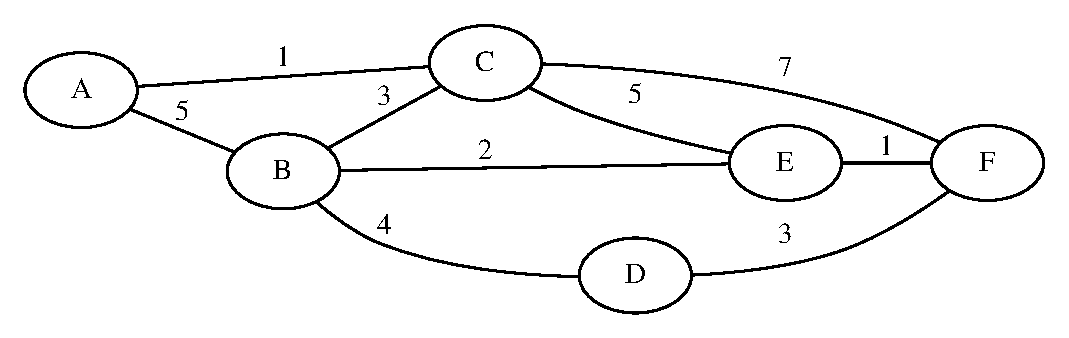
\includegraphics[scale=0.5]{dji.eps}
		\end{center}
		\begin{tabularx}{\textwidth}{|X|X|X|X|X|X|X|}
			\hline
			A                                        & B                                         & C                                        & D                                      & E                                         & F                                         &                                    \\
			\hline
			\alt<2->{ 0 (A)}{ }                      & \alt<4->{5 (A)}{}                         & \alt<5->{1 (A)}{ }                       &                                        &                                           &                                           & \alt<3->{ \textcolor{blue}{A}}{ }  \\
			\hline
			\alt<3->{\textcolor{blue}{\ding{52}}}{ } & \alt<8->{4 (C)}{ }                        & \alt<6->{\textcolor{red}{1 (A)}}{ }      &                                        & \alt<9->{6 (C)}{ }                        & \alt<10->{8 (C)}{ }                       & \alt<7->{ \textcolor{blue}{C}}{ }  \\
			\hline
			\alt<3->{\textcolor{blue}{\ding{52}}}{ } & \alt<11->{\textcolor{red}{4 (C)}}{ }      & \alt<7->{\textcolor{blue}{\ding{52}}}{ } & \alt<13->{8 (B)}{ }                    & \alt<14->{6 (B)}{ }                       & \alt<14->{8 (C)}{ }                       & \alt<12->{ \textcolor{blue}{B}}{ } \\
			\hline
			\alt<3->{\textcolor{blue}{\ding{52}}}{ } & \alt<12->{\textcolor{blue}{\ding{52}}}{ } & \alt<7->{\textcolor{blue}{\ding{52}}}{ } & \alt<18->{8 (B)}{ }                    & \alt<15->{\textcolor{red}{6 (B)}}{ }      & \alt<17->{7 (E)}{}                        & \alt<16->{ \textcolor{blue}{E}}{ } \\
			\hline
			\alt<3->{\textcolor{blue}{\ding{52}}}{ } & \alt<12->{\textcolor{blue}{\ding{52}}}{ } & \alt<7->{\textcolor{blue}{\ding{52}}}{ } & \alt<21->{8 (B)}{ }                    & \alt<16->{\textcolor{blue}{\ding{52}}}{ } & \alt<19->{\textcolor{red}{7 (E)}}{ }      & \alt<20->{ \textcolor{blue}{F}}{ } \\
			\hline
			\alt<3->{\textcolor{blue}{\ding{52}}}{ } & \alt<12->{\textcolor{blue}{\ding{52}}}{ } & \alt<7->{\textcolor{blue}{\ding{52}}}{ } & \alt<22->{\textcolor{red}{{8 (B)}}}{ } & \alt<16->{\textcolor{blue}{\ding{52}}}{ } & \alt<19->{\textcolor{blue}{\ding{52}}}{ } & \alt<23->{ \textcolor{blue}{D}}{ } \\
			\hline
		\end{tabularx}
	\end{exampleblock}
\end{frame}


\begin{frame}
	\mframe{\Reseau}
	\begin{exampleblock}{Algorithme de Dijkstra}
		\begin{center}
			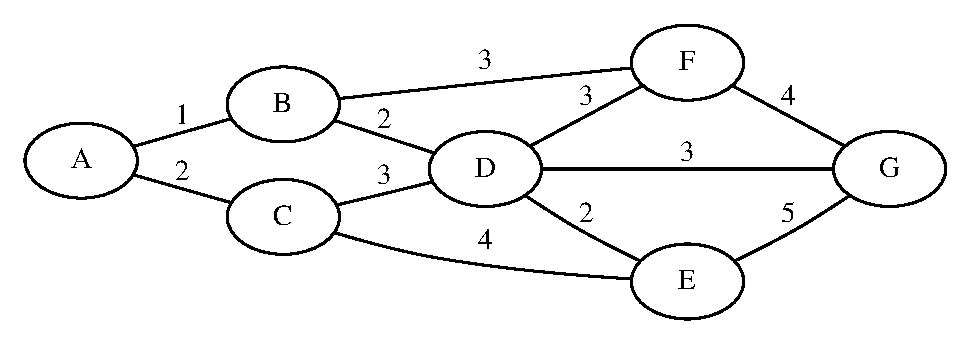
\includegraphics[scale=0.5]{monka.eps}
		\end{center}
		\begin{tabularx}{\textwidth}{|X|X|X|X|X|X|X|X|}
			\hline
			A & B & C & D & E & F & G & \\
			\hline
			  &   &   &   &   &   &   & \\
			\hline
			  &   &   &   &   &   &   & \\
			\hline
			  &   &   &   &   &   &   & \\
			\hline
			  &   &   &   &   &   &   & \\
			\hline
			  &   &   &   &   &   &   & \\
			\hline
			  &   &   &   &   &   &   & \\
			\hline
			  &   &   &   &   &   &   & \\
			\hline
		\end{tabularx}
	\end{exampleblock}
\end{frame}

\end{document}